\documentclass[runningheads,a4paper]{llncs}

\usepackage{amssymb}
\setcounter{tocdepth}{3}
\usepackage{graphicx}
\usepackage{subfigure}
\usepackage{color}
\usepackage{amsmath}

\long\def \ignore#1{}
\newcommand{\tk}[1]{{\bf {\textcolor{magenta}{#1 -- TK}}}}
\newcommand{\hg}[1]{{\bf {\textcolor{red}{#1 -- HG}}}}
\newcommand{\keywords}[1]{\par\addvspace\baselineskip
\noindent\keywordname\enspace\ignorespaces#1}
\newcommand{\goodgap}{
        \hspace{\subfigtopskip}
        \hspace{\subfigbottomskip}}

\renewcommand{\baselinestretch}{1.5}

\begin{document}

\mainmatter 

\title{PARC: Edge Probability Assignment in Signaling Networks through
Reachability and Coexpression}

\titlerunning{PARC: Probability Assignment through Reachability \&
Coexpression}

\author{Haitham Gabr\inst{1} \and Juan Carlos Rivera-Mulia\inst{2} \and David M
Gilbert\inst{2} \and Tamer Kahveci\inst{1}}

\authorrunning{Gabr et al.}


\institute{Department of Computer \& Information Science \& Engineering,\\
University of Florida,\\
Gainesville, Florida 32611, USA\\
\and
Department of Biological Science,\\
Florida State University,\\
Tallahassee, Florida 32306, USA\\}

\maketitle


\begin{abstract}
Abstract here.
\end{abstract}

\section{Introduction}

Recent literature exhibits a great interest in studying biological networks.
These networks model collaboration between different molecules, such as
proteins, to carry out various cellular functions. Interacting molecules are
often modeled as nodes, while their interactions are modeled as edges which
connect these nodes.
Studying biological networks has proven to be highly important. It gives us deep
insight into cellular mechanics and allows us to understand how biological
processes are maintained. Discovering signaling
pathways~\cite{missing}, mapping transcription regulation~\cite{missing}, and
identifying the reasons behind and the consequences of various
disorders~\cite{missing}, are only a few examples of many other applications
which are possible through studying biological networks.

One of the critical factors that affects our analysis of biological networks is
that their topologies are usually uncertain. This uncertainty follows from the
fact that key biological processes governing these interactions, like DNA
replication and gene expression, are themselves inherently uncertain.
For instance, research shows that DNA replication can start at different
chromosome locations with different probabilities~\cite{missing}. It also shows that different
biological processes like gene replication timing, expression and
transcription regulation vary across different cell types~\cite{missing}, and
also from healthy cases to different disorders~\cite{missing}. Probabilistic
networks model this uncertainty in a mathematically sound manner~\cite{missing}.
Briefly, a probabilistic biological network represents each edge with a
probability value indicating the chance that the accociated interaction
actually takes place.

Taking the interaction probabilities into account is extremely important in
studying networks as they improve the accuracy of the results, and can lead to
biologically significant observations that are impossible to achieve otherwise.
A few examples of the applications that utilize interaction probabilities
include signaling pathway detection~\cite{missing}, characetrizing the network
topology~\cite{missing}, signal reachability~\cite{missing}, node centrality,
and network stability~\cite{missing}. Therefore, having accurate knowledge of
interaction probabilities is of utmost importance. It is also imperative to gain
knowledge about phenotype-specific interaction probabilities in order to obtain
phenotype-specific results. For example, Analysis of a biological network in a
specific cell type or under a given disorder depends on the knowledge of the
network edge probabilities in this specific cell type or disorder.

In the literature, probability values were assigned to edges of biological
networks in multiple ways. Interaction databases like MINT~\cite{missing} and 
STRING~\cite{missing} provide a confidence value for each interaction that
represents the level of certainty in observing this interaction. This way of
probability assignment compensates for the level of noise in the experiment used
to observe the interaction. However, it does not account for the inherent
stochasticity of the interaction events. Sharan {\it et al.}~\cite{log_reg}
utilized features like the volume of evidence present for the interaction, gene
expression correlation, and network topology to learn the interaction
probabilities. Incorporating gene expression correlation in this model serves
the inherent interaction uncertainty to some extent. However, it only accounts
for the correlation between the interacting gene products, ignoring their
relations with the rest of the network. Thus, new methods which can compute
interaction probabilities by taking the entire network into consideration is
needed.

{\bf Contributions.} In this paper, we present a novel method for computing edge
probabilities for a given signaling networks topology. We use end-to-end
signal reachability values as the main guide for our computation. While it is
hard to observe the probability of each individual interaction on a micro level,
target reachability values are much easier to observe on a macro level.
Moreover, they can be observed in different cell types or under different
disorders, paving way for computing phenotype-specific edge probabilities.

Gene expression correlation has been widely used as primary evidence for
signaling and regulation~\cite{missing}. Here, we rely on gene expression
correlation as a guide for source-target signal reachability. For every pair of
source (receptor) and target (reporter) nodes, we compute a normalized Pearson
correlation value between their gene expression levels, and use these values as
input to our method.

Given the source-target reachability values, our method uses them as an
objective and optimizes the edge probability values so that the computed
reachability values are as close as possible to this objective. Given a network
with $n$ edges, reachability probability can be expressed as an $n$th degree
function of $n$ variables~\cite{preach}. Optimizing this function in an exact
manner would require solving a system of $n$ simultaneous derivative equations.
The key challenge arises from the fact that computing the function itself has an
exponential time complexity, equivalent to computing all combinations of $n$ objects. This makes exact
optimization impossible for medium to large sized networks.

Instead of exact optimization, we develop a two-phase strategy. The first phase
is global optimization using a genetic algorithm, where we search the entire
space for a good starting point of the edge probabilities. The second phase is
local optimization using hill climbing, where we enhance our starting point to
reach an optimum set of probabilities. Furthermore, instead of optimizing all
$n$ variables simultaneously, we seek to optimize the iteratively; at each
step, we consider only one edge probability for optimization, fixing all other
values. We show that our method produces a result that is very close to the
objective.

We demonstrate the capacity of our method by computing the edge probabilities
for signaling networks of different leukemia subtypes. We present biological
validation results by identifying specific genes and interactions that are
characteristic to specific leukemia subtypes.

The rest of this paper is organized as follows. Section~\ref{sec:method}
details the method. Section~\ref{sec:results} discusses our results.
Section~\ref{sec:conc} concludes the paper.

\section{Method}
\label{sec:method}

In this section we explain in detail our method for computing edge probability
values of a probabilistic signaling network. Our method consists of two phases:
global optimization and local optimization. In Section~\ref{subsec:def} we start
by describing some preliminaries and formally definig the problem. In
Section~\ref{subsec:single} we explain an important cornerstone of phase 2.
Sections \ref{subsec:phase1} and \ref{subsec:phase2} explain the method in
detail.

\subsection{Preliminaries}
\label{subsec:def}
Through the rest of the paper we define a probabilistic signaling network as a
graph $G = (V, E, P)$, where $V$ denotes the set of nodes (i.e., genes), $E$
denotes the set of edges (i.e., interactions), and $P: E \rightarrow [0, 1]$
denotes a function that returns the existence probability of each edge in $E$.
We also define the two sets $S \subseteq V$ and $T \subseteq V$ as the sets of
source nodes (i.e., receptor genes) and target nodes (i.e., reporter genes). We
define the function $C: S \times T \rightarrow [0, 1]$ as a gene coexpression
function that returns the absolute value of the Pearson correlation coefficient
between the gene expression of $(s, t)$, where $s \in S$ and $t \in T$. We
define the function $R: S \times T \rightarrow [0, 1]$ as the signal
reachability function that returns the probability of a signal propagating successfully from
$s$ to $t$, where $s \in S$ and $t \in t$. Notice that the knowledge of $R$
depends on that of $P$~\cite{preach}.

\paragraph{\textbf{Problem definition.}} Given $V$, $E$, $S$, $T$, and $C$, Find
$P$ such that $\|D\|$ is minimum, where $D$ is a difference vector formed by
listing the values of $C(s, t) - R(s, t) \forall (s, t) \in S \times T$.

The method we develop to solve this problem relies on solving a modified version
of the reachability problem. In the reachability problem, $P$ is known and the
goal is to find $R$, while in the problem detailed above the goal is to find $P$
based on $C$ as a guide for $R$. Following is a brief description of the PReach
method that solves the reachability problem. We refer the readed to its paper
for more elaborate description and examples~\cite{preach}.

Let $U = \{1, \ldots, n\}$, where $n = |E|$. Let $X$ and $Y$ be two sets of $n$
variables, where $X = \{x_1, \ldots, x_n\}$ and $Y = \{y_1, \ldots, y_n\}$. Let
$\Theta$ be a subset of $U$. Let $S_1, \dots, S_k$ be $k$ different subsets of
$\Theta$. Let $x_{S_i} = \prod_{j \in S_i}x_j$ and $y_{S_i} = \prod_{j \in
S_i}y_j$, where $i \in \{1, \ldots, k\}$. Let $x^*$ and $y^*$ be two free
variables. Let $a_1, \ldots, a_k, b$ and $c$ be real numbers. PReach defines an
\emph{\textbf{xy-polynomial}} over $\Theta$ as $F =
\sum_{i=1}^k{a_i}x_{S_i}y_{\Theta \setminus S_i} + bx^* + cy^*$. Except for the
free variables, each term in the above summation contains each of the indices
$j \in \Theta$ either as a product term $x_j$ or $y_j$.

PReach associates every edge $e_j \in E$ with a variable $x_j \in X$ and a
variable $y_j \in Y$, where $j \in U$. $x_j$ represents the case where $e_j$ is
present, while $y_j$ represents the case where $e_j$ is absent. In the above
summation, each of the non-free terms ${a_i}x_{S_i}y_{\Theta \setminus S_i}$
represents a combination where $e_j$ is present $\forall j \in S_i$ and absent
$\forall j \in \Theta \setminus S_i$. $a_i$ designates the probability of this
specific combination. The free variable $x^*$ represents the case where $T$ is
reachable from $S$, and $b$ designates its probability. Inversely, The free
variable $y^*$ represents the case where $T$ is unreachable from $S$, and $c$
designates its probability.

Let $p_i = P(e_i)$ and $q_i = 1-p_i$. PReach starts by associating every edge
$e_i \in E$ with a binomial $p_i x_i + q_i y_i$. It then proceeds by
multiplying these binomials together into a growing $xy$-polynomial. After every multiplication
step, PReach checks the polynomial for non-free terms that can be
\emph{collapsed} into one of the two free terms as follows. For any of the
non-free terms ${a_i}x_{S_i}y_{\Theta \setminus S_i}$, if the edges associated
with $S_i$ form at least one path from $S$ to $T$, the term is replaced by
$a_i x^*$. Inversely, if the edges associated with ${\Theta \setminus S_i}$ form
at least one cut between $S$ and $T$,  the term is replaced by $a_i y^*$. Any
further multiplication of a new term $p_i x_i$ with $b x^*$ results in $b p_i
x^*$. Similarly, $(p_i x_i)(c y^*) = c p_i y^*$, $(q_i y_i)(b x^*) = b q_i x^*$,
and $(q_i y_i)(c y^*) = c q_i y^*$. Hence, the size of the $xy$-polynomial
avoids growing in an exponential rate.



\subsection{Optimizing a single edge probability}
\label{subsec:single}

In this section we describe a building block of our method, which is how we
optimize a single edge probability. This is a crucial part of our method that we
will refer to in Section~\ref{subsec:phase2}. Let us assume that for only one
edge $e \in E$, its probability $p_e$ is unknown. Assume that the probability
values of all other edges in $E - \{e\}$ are known. How do we compute the value
of $p_e$ that serves the global purpose of solving the problem described in
Section~\ref{subsec:def}?

For this purpose, we introduce a modification for the PReach
method~\cite{preach}. Originally, PReach computes the reachability probability
between two nodes in the network given that all edge probability values are
known. It works by assigning a binomial to every edge based on its probability,
and multiplying all the binomials together to form a complex polynomial. Terms
in this polynomial describes all possible combinations of edge presence.
Reachability probability is the sum of coefficients of the terms representing
reachable combinations. We modify the method by making it accept one of the edge
probabilities $p_e$ as unknown. We defer the multiplication of the binomial
representing $e$ to the end. As a result, instead of outputting a number,
PReach outputs the reachability probability in terms of $p_e$ as $\alpha +
\beta p_e$, where $\alpha$ and $\beta$ are numbers.

We proceed by computing $R(s, t) = \alpha_{st} + \beta_{st} p_e \forall
(s, t) \in S \times T$. Based on the global goal of minimizing $\|D\|$,
following is a deduction of the optimal value for $p_e$:

\begin{align*}
&Minimize~~~\|D\| = \sum_{(s,t) \in S \times T} [C(s, t) - R(s, t)]^2\\
&			   = \sum_{(s,t) \in S \times T} [C(s, t) - \alpha_{st} -
			   \beta_{st} p_e]^2\\
&therefore\\
&\frac{d}{dp_e} \sum_{(s,t) \in S \times T} [C(s, t) - \alpha_{st} -
			   \beta_{st} p_e]^2 = 0\\
&\sum_{(s,t) \in S \times T} -2\beta_{st} [C(s, t) - \alpha_{st} -
\beta_{st} p_e] = 0\\
&\sum_{(s,t) \in S \times T} -2\beta_{st} [C(s, t) - \alpha_{st}] + p_e
\sum_{(s,t) \in S \times T} 2\beta_{st}^2 = 0\\
&p_e = \frac{\sum_{S \times T} \beta_{st} [C(s, t) -
\alpha_{st}]}{\sum_{S \times T} \beta_{st}^2}\\
\end{align*}

The formula above constitutes the optimal value for $p_e$ given all other
probability values. However, there is no guarantee it must fall within the
proper probability range of $[0, 1]$. If it does not, we move it to the closest
limit of the proper range. If it is above $1$, we replace it with $1$. If it
is below $0$, we replace it with $0$.

\subsection{Phase 1: global optimization}
\label{subsec:phase1}

The first phase of our method is a global optimization phase through a genetic
algorithm. The two key definitions of a genetic algorithm are the format of a
candidate solution and its fitness function. For our genetic algorithm, we
define a candidate solution $\psi$ as a vector of the edge probability values
listed in a fixed edge order. We define the fitness $F_{\psi}$ of a candidate
solution $\psi$ as $\|D\|/|E|$, where $D$ is the difference vector explained in
Section~\ref{subsec:def}, computed using the probability values from $\psi$.

\paragraph{\textbf{Initialization.}} We start by generating a set $Q$ of 50
random candidate solutions to form the seed population. We generate each seed candidate
solution $\psi$ by assigning a random number between 0 and 1 to each of its
entries. We then compute the fitness values $F_{\psi} \forall \psi \in Q$.

\paragraph{\textbf{Crossover.}} We randomly select two solutions $\psi_1$ and
$\psi_2$ from $Q$ to crossover. Every solution has a chance of being selected that is
directly proportional to its fitness. We compute a \emph{gap} value for each of
$\psi_1$ and $\psi_2$, which is the sum of all values in $D$. Since the
difference vector $D$ represents the difference between the target values $C(s,
t)$ and the current values $R(s, t)$, we classify $\psi$ as \emph{deficit} if
it has a positive gap (i.e., $R < C$). Inversely, we classify $\psi$ as
\emph{surplus} if it has a negative gap (i.e., $R > C$). We use $\psi_1$ and
$\psi_2$ to generate a child candidate solution as follows. For every entry $i
\in \{1, .., |E|\}$, we choose either entry $\psi_{1i}$ or $\psi_{2i}$ based on
which is more likely to produce a candidate solution with a higher fitness. If
both $\psi_1$ and $\psi_2$ are deficit, we choose the higher of $\psi_{1i}$ or
$\psi_{2i}$. Inversely, if both $\psi_1$ or $\psi_2$ are surplus, we choose the
lower of $\psi_{1i}$ or $\psi_{2i}$. If one of $\psi_1$ and $\psi_2$ is deficit
and the other is surplus, then we randomly select between $\psi_{1i}$ and
$\psi_{2i}$, where the chances of each is directly proportional to the fitness
of their containing solutions. This scheme as a whole increases the chances of
the resulting candidate solution having a higher fitness. We repeat the
crossover step 50 times and add the resulting new candidate solutions to $Q$.

\paragraph{\textbf{Mutation.}} For every candidate solution $\psi \in Q$, we
iterate over every entry $\psi_i$. For every given entry $\psi_i$, we perform a
Bernoulli trial with probability of 0.01. If the trial yields success, the
entry value is replaced with a new value drawn uniformly at random from the
range [0, 1].

\paragraph{\textbf{Selection.}} From the 100 candidate solutions in $Q$, we
select five solutions with the highest fitness values. Additionally, we randomly select
another 45 solutions from the remaining 95, where every solution has a chance
of selection that is directly proportional to its fitness. We exclude the
non-selected 50 soultions from $Q$.

We repeat the crossover, mutation and selection steps 100 times. We then select
the candidate solution with the highest fitness as the output of this phase. We
use it as an input to our next local optimization phase.

\subsection{Phase 2: local optimization}
\label{subsec:phase2}

In this phase we employ a hill climbing scheme for local optimization. We start
with the top candidate solution $\psi$ obtained from phase 1 and iteratively
update it until a local optimum is reached. To complete one update to the
solution, we iteratively compute a new value for each individual edge
probability that is optimal with respect to all other edge probabilities.

We start by choosing any edge $e \in E$. We assume its probability $\psi_e$ is
unknown, while probabilities of all edges in $E - \{e\}$ are fixed to their
current values. We then calculate the optimal value of $\psi_e$ as explained in
Section~\ref{subsec:single}. We record the value $\delta_e$ as the difference
between the old and new values of $\psi_e$. We repeat this step for all $e \in
E$. We then repeat the whole process until $\delta_e \approx 0$ for all $e \in
E$.
We output the final value of $\psi$ as the problem solution.


\section{Experimental results}
\label{sec:results}

In this section we show experimental results for computing edge probability
values for some signaling networks from KEGG. We also show comparative
analysis of these values across different leukemia subtypes. We obtained the
gene expression samples for the leukemia subtypes from Zhang {\it et
al.}~\cite{mullighan}. Based on the computed edge probability values, we also
compute different gene centrality values for the networks across these leukemia
subtypes. We extract the genes that behave differently in a specific pair
of network and leukemia subtype, and analyze the significance of these genes in
this pair. Our results provide an insight into the relation between specific
signaling networks and leukemia subtypes, as well as similarities among leukemia
subtypes.

\subsection{Edge probability under different leukemia subtypes}
\label{sec:results:edge}

In this experiment, we explore the differences in signaling among seven leukemia
subtypes. We want to know how different edge probabilities are across these
subtypes, and whether an edge exhibits a relatively different probability in a
specific subtype. To achieve this, We used our method to compute edge
probability values for four KEGG signaling networks. For each network, we ran
our method seven times. At each time, we used gene expression data for a
different leukemia subtype. As a result, for every network, we have a different
probability value for every edge in every leukemia subtype. We obtained a
hierarchical clustering of edges and subtypes for every network.
Figure~\ref{fig:prob_cluster} shows the results.

\begin{figure}[t]
\centering
\subfigure[Apoptosis]
{\includegraphics[width=0.46\textwidth]{figures/edges/apoptosis.png} }
\goodgap
\subfigure[Cell cycle]
{\includegraphics[width=0.46\textwidth]{figures/edges/cellcycle.png} }
\goodgap
\subfigure[Complement \& coagulation]
{\includegraphics[width=0.46\textwidth]{figures/edges/ccc.png} }
\goodgap
\subfigure[Chemokine]
{\includegraphics[width=0.46\textwidth]{figures/edges/chemokine.png} }
\caption{Edge probability values in different leukemia subtypes. Rows represent
leukemia subtypes, and columns represent network edges.}
\label{fig:prob_cluster}
\end{figure}

From the figure we observe that the probability value of some edges vary
aggressively across different leukemia subtypes. For instance, CASP3 is the
target in three different Apoptosis interactions whose probability in a
subtype is at least 2 standard deviations away from their mean values among
other subtypes. These interactions are (CASP10 $\rightarrow$ CASP3) in
Hyperdiploid, (CASP12 $\rightarrow$ CASP3) in T-ALL, and (BIRC8 $\rightarrow$
CASP3) in Ph. Similarly, CHEK1 is the source in two different Cell cycle
interactions whose probability in a subtype is at least 2 standard deviations
away from their mean values among other subtypes. These interactions are (CHEK1
$\rightarrow$ CDC25A) in T-ALL, and (CHEK1 $\rightarrow$ TP53) in MLL. CASP3
is already linked to B-cell lymphoma~\cite{casp3_lymphoma},
lung~\cite{casp3_lung}, skin~\cite{casp3_skin}, breast~\cite{casp3_breast}, and
other cancers. CHEK1 is linked to oral squamous cell
carcinoma~\cite{chek1_oral} and colorectal cancer~\cite{chek1_colorectal}. Our
observation makes both genes strong candidates for investigation in their
respective subtypes of leukemia.

Additionally, the hierarchy of the leukemia subtypes gives an insight about
which subtypes have similar signaling behavior in each network. T-ALL and
TCF3-PBX1 are closest to each other in Apoptosis, Complement \& coagulation and
Chemokine, noticeably more distant in Cell cycle. Hyperdiploid is very similar
to TCF3-PBX1 in Cell cycle, but more distant from it in the other three
networks. In fact, Hyperdiploid is the most distant from all other subtypes in
both Apoptosis and Chemokine.

\subsection{Gene centrality under different leukemia subtypes}
Next, we use the edge probability values we computed in
Section~\ref{sec:results:edge} to compute centrality values of the genes in
each network using the method in Gabr {\it et al.}~\cite{preach_bio}.
We compute a centrality of a gene as the drop in reachability probability when
the gene is removed from the network. Similar to
Section~\ref{sec:results:edge}, We compute centrality values for the genes of
the same four networks. For each network, we computed gene centrality for
its seven versions designated by the leukemia subtypes. As a result, For every
network, we have a different centrality value for every gene in every leukemia
subtype. We obtained a hierarchical clustering of genes and subtypes for every
network. Figure~\ref{fig:cent_cluster} shows the results.

\begin{figure}[t]
\centering
\subfigure[Apoptosis]
{\includegraphics[width=0.46\textwidth]{figures/centrality/apoptosis.png} }
\goodgap
\subfigure[Cell cycle]
{\includegraphics[width=0.46\textwidth]{figures/centrality/cellcycle.png} }
\goodgap
\subfigure[Complement \& coagulation]
{\includegraphics[width=0.46\textwidth]{figures/centrality/ccc.png} }
\goodgap
\subfigure[Chemokine]
{\includegraphics[width=0.46\textwidth]{figures/centrality/chemokine.png} }
\caption{Gene centrality}
\label{fig:cent_cluster}
\end{figure}

The figure shows a variation of centrality value for some genes across different
leukemia subtypes. However, this variation is not as diverse as that of edge
probability values addressed in Section~\ref{sec:results:edge}. Still, some
genes have a centrality value in a specific leukemia subtype that is noticeably
different from its value in other subtypes. In Apoptosis, BID is the top
outstanding genes in Hyperdiploid, with centrality values 2.8 standard
deviations higher than their mean centrality in other sub ypes. RIPK1 and CASP7
have significantly lower centrality in ETV6\_RUNX1 and Ph respectively than
other subtypes. In Cell cycle, CDK1 and PLK1 are the top outstanding genes in
Hypo, with centrality values 2.6 standard deviations higher than their mean
centrality in other subtypes. BID is linked to leukemia~\cite{bid_leukemia} and
other cancers. RIPK1 and CASP7 are linked to colorectal
cancer~\cite{ripk1_casp7}. CDK1 amd PLK1 are also linked to
leukemia~\cite{cdk1_plk1_leukemia}, as well as other cancers like
mesothelioma~\cite{cdk1_plk1_meso} and breast
cancer~\cite{cdk1_breast,plk1_breast}. Based on our observations, these genes
are interesting targets for studying in the scope of their respective leukemia
subtypes.

\subsection{Enrichment analysis of outstanding genes}

Following from the previous results, we want to know which network plays a
key role in a certain leukemia subtype. In other words, we want to know which
network's outstanding set of genes is highly enriched in a specific leukemia
subtype. To achieve this, we first extract the set $L$ of outstanding genes for
every network in every subtype. For every edge $e = (u,v)$ in a given network,
we computed the mean $\mu_e$ and standard deviation $\sigma_e$ of its
probability values in all leukemia subtypes. Then for every subtype, for every
edge $e$, we checked if the probability of $e$ in this subtype was at least
$2\sigma_e$ away from $\mu_e$. If it was, we added $u$ and $v$ to $L$. we then
performed gene set enrichment analysis (GSEA)~\cite{gsea} on $L$ for every
network in every leukemia subtype. For every pair of network and subtype, we
set the phenotype $A$ as the subtype samples, and phenotype $B$ as all samples
from other subtypes. We then ran GSEA on the network's outstanding gene set $L$
to measure its differential significance from $A$ to $B$. We considered gene
sets whose $p$ value is above 0.1 as highly enriched. Table~\ref{tab:gsea_edge}
lists these gene sets and their $p$ values in their respective leukemia
subtypes. Figure~\ref{fig:gsea_edge} shows the gene set enrichment plots for the
two highest enriched gene sets.


\begin{table}[t]
\centering
\caption{Signaling networks with a highly enriched gene set in a leukemia
subtype.}
\label{tab:gsea_edge}
\begin{tabular}{|l|l|l|l|}
\hline
Subtype & Network & $p$ value & Gene set \\ \hline
Hyperdiploid & Apoptosis & 0.0083 & \scriptsize{NFKB1, RELA, BCL2, PPP3CA,
PPP3CB, PPP3CC,} \\
 & & & \scriptsize{PPP3R1, BAD, AKT3, AKT1, AKT2, CHUK,} \\
 & & & \scriptsize{IKBKB, IKBKG, CASP7, DFFA, CASP10, CASP3,} \\
 & & & \scriptsize{IL3, CSF2RB, IL3RA, TNF, TNFRSF1A} \\
\hline
ETV6\_RUNX1 & Cell cycle & 0.0151 & \scriptsize{TFDP1, TFDP2, E2F1, RBP3, E2F2,
E2F3,} \\
& & & \scriptsize{CCNE1, CCNE2, CDK4, CDK6, CCND1, CCND2,} \\
& & & \scriptsize{CCND3, RBL1, PRB1, RBL2, CDK2, CCNA2,} \\
& & & \scriptsize{CCNA1} \\
\hline
T-ALL & Apoptosis & 0.0162 & \scriptsize{BIRC2, BIRC3, XIAP, BIRC7, CASP7,
NFKB1,} \\
& & & \scriptsize{RELA, CASP3, DFFA, FADD, CASP8, IL1R1,} \\
& & & \scriptsize{IL1RAP, TRADD, FASLG, FAS} \\
\hline
TCF3-PBX1 & Apoptosis & 0.0167 & \scriptsize{PRKACA, PRKACB, PRKACG, PRKAR1A,
PRKAR1B,} \\
& & & \scriptsize{PRKAR2A, PRKAR2B, PRKX, BAD, IL1A, IL1B, IL1R1,} \\
& & & \scriptsize{IL1RAP, TNFRSF10D, TNFRSF10C, TNFRSF10B, FADD} \\
\hline
Hypo & Apoptosis & 0.0484 & \scriptsize{CAPN1, CAPN2, IRAK3, IRAK1, IRAK4,
MAP3K14,} \\
& & & \scriptsize{BCL2, TP53, NGF, NTRK1} \\
\hline
Ph & Cell cycle & 0.088 & \scriptsize{BUB1, BUB3, CDKN2A, CDK4, CDK6, CCND1,}\\
& & & \scriptsize{CCND2, CCND3, RB1, CDC45L, MCM7, MCM2,} \\
& & & \scriptsize{MCM6, MCM5, MCM4, MCM3, CCNL1, LAT,} \\
& & & \scriptsize{ORC3L, ORC5L, ORC4L, ORC2L, ORC1L, ORC6L,} \\
& & & \scriptsize{CDC2, CCNA2, CCNA1, CDKN1B, CDKN1C, CDK2,} \\
& & & \scriptsize{CDC25A, CDKN1A, CCNE1, CCNE2, TP53, GADD45G,} \\
& & & \scriptsize{GADD45A, GADD45B} \\
\hline
\end{tabular}
\end{table}


\begin{figure}[t]
\centering
\subfigure[Apoptosis in Hyperdiploid]
{\includegraphics[width=0.46\textwidth]{figures/gsea/edge_apoptosis_hyperdiploid.png}
}
\goodgap
\subfigure[Cell cycle in ETV6\_RUNX1]
{\includegraphics[width=0.46\textwidth]{figures/gsea/edge_cellcycle_etv.png} }
\caption{Gene set enrichment plots for the highest two enriched gene sets in
their respective leukemia subtypes.}
\label{fig:gsea_edge}
\end{figure}

We observe from Table~\ref{tab:gsea_edge} that Apoptosis and Cell cycle
signaling networks are dominant in all gene sets that are highly enriched. This
implies a fundamental role for these two networks in the listed subtypes. It
also implies that these subtypes are either caused by or leading to a
perturbation in their respective gene sets. Another noteworthy observation is
that, although all the highly enriched gene sets belong to only two networks,
there are little overlap between them. In Apoptosis for instance, PPP3 genes are
dominant in Hyperdiploid, while BIRC genes are dominant in T-ALL, and PRKA genes
are dominant in TCF3-PBX1. Additionally, from Figure~\ref{fig:gsea_edge} we
observe that, although Apoptosis and Cell cycle have the highest enriched gene
sets for Hyperdiploid and ETV6\_RUNX1 respectively, their relations to their
respective leukemia subtypes are not the same. All genes in the Apoptosis set in
Hyperdiploid exhibit higher expression than in other subtypes, which implies
up-regulation of these genes in Hyprediploid. On the other hand, most of the
genes in the Cell cycle set in ETV6\_RUNX1 have lower expression than in other
subtypes, which indicates down-regulation of these genes in ETV6\_RUNX1.

\section{Conclusion}
\label{sec:conc}

Conclusion here

\section*{Acknowledgement}
Ack here.

\bibliographystyle{plain}%
\bibliography{ref}


\end{document}
